\begin{figure}[t]
    \centering
    \begin{subfigure}[t]{0.32\textwidth}
        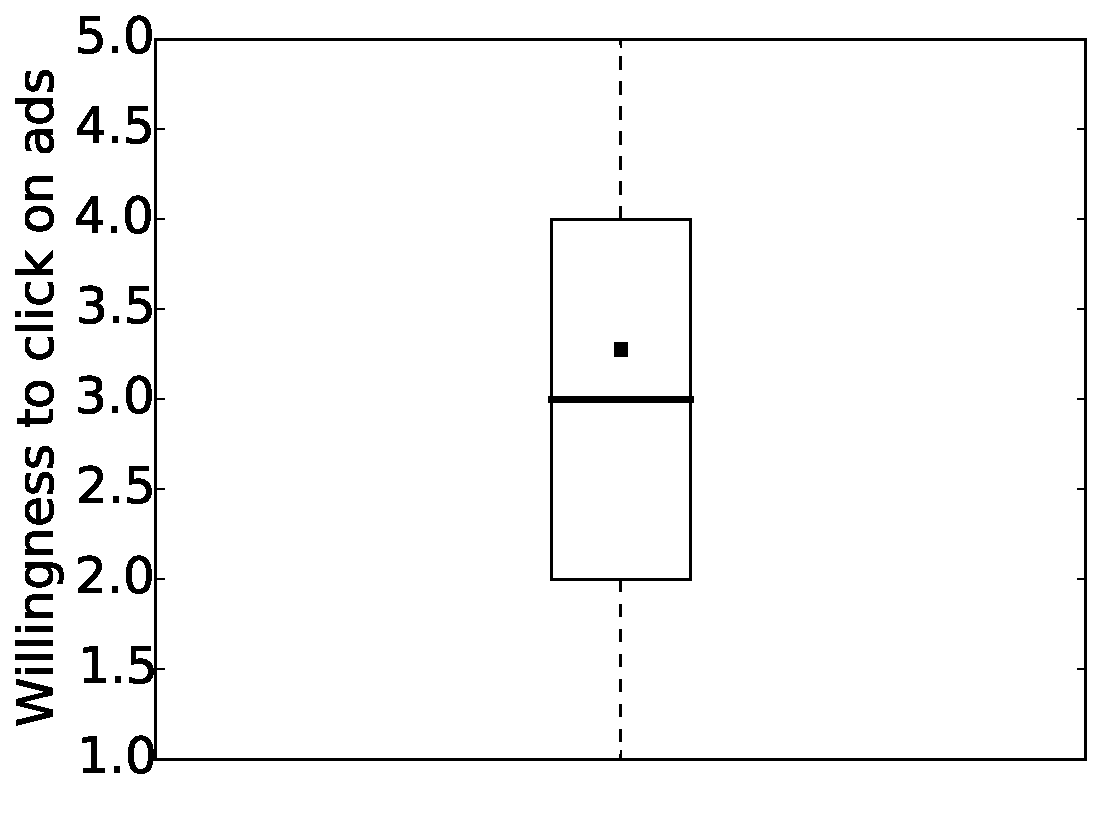
\includegraphics[width=\textwidth]{adinjection/figures/user_study/clicking.pdf}
        \caption{\scriptsize{Susceptibility to ad injection.}}
        \label{adinjection:fig:eval:user_study:susceptibility}
    \end{subfigure}
    \hfill
    \begin{subfigure}[t]{0.32\textwidth}
        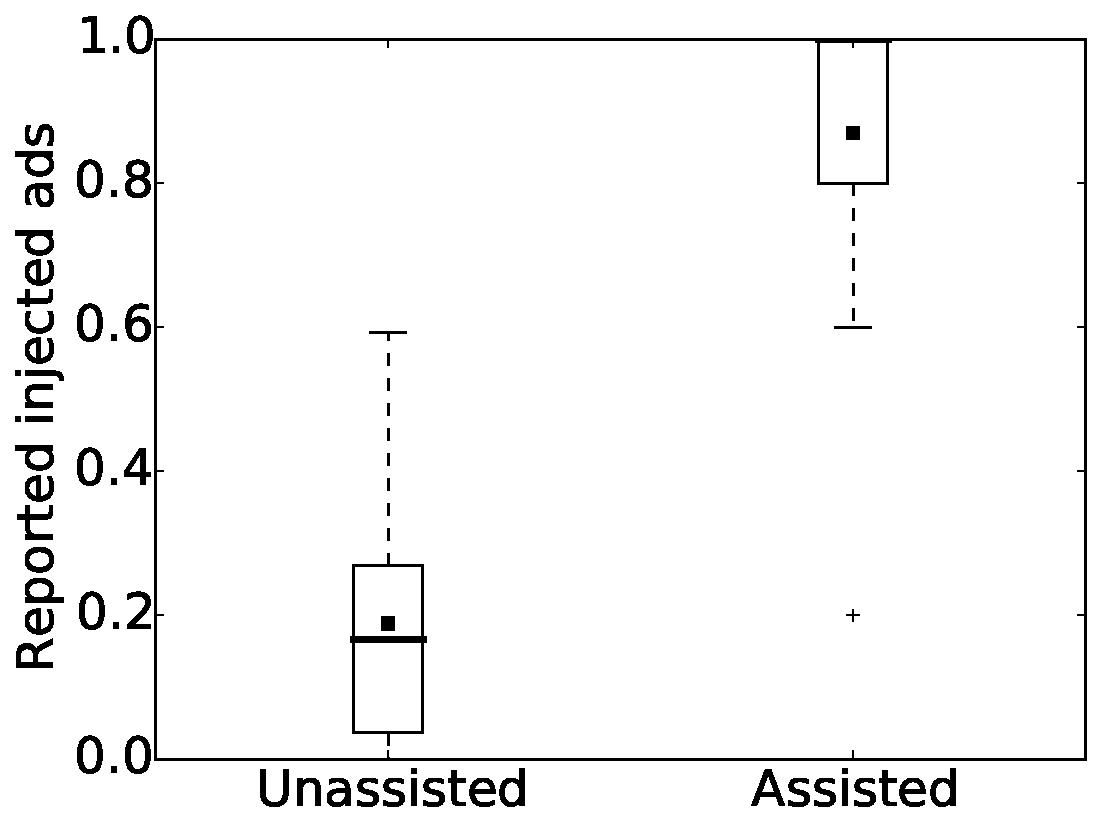
\includegraphics[width=\textwidth]{adinjection/figures/user_study/identification.pdf}
        \caption{\scriptsize{Ability to identify injected ads.}}
        \label{adinjection:fig:eval:user_study:identification}
    \end{subfigure}
    \hfill
    \begin{subfigure}[t]{0.32\textwidth}
        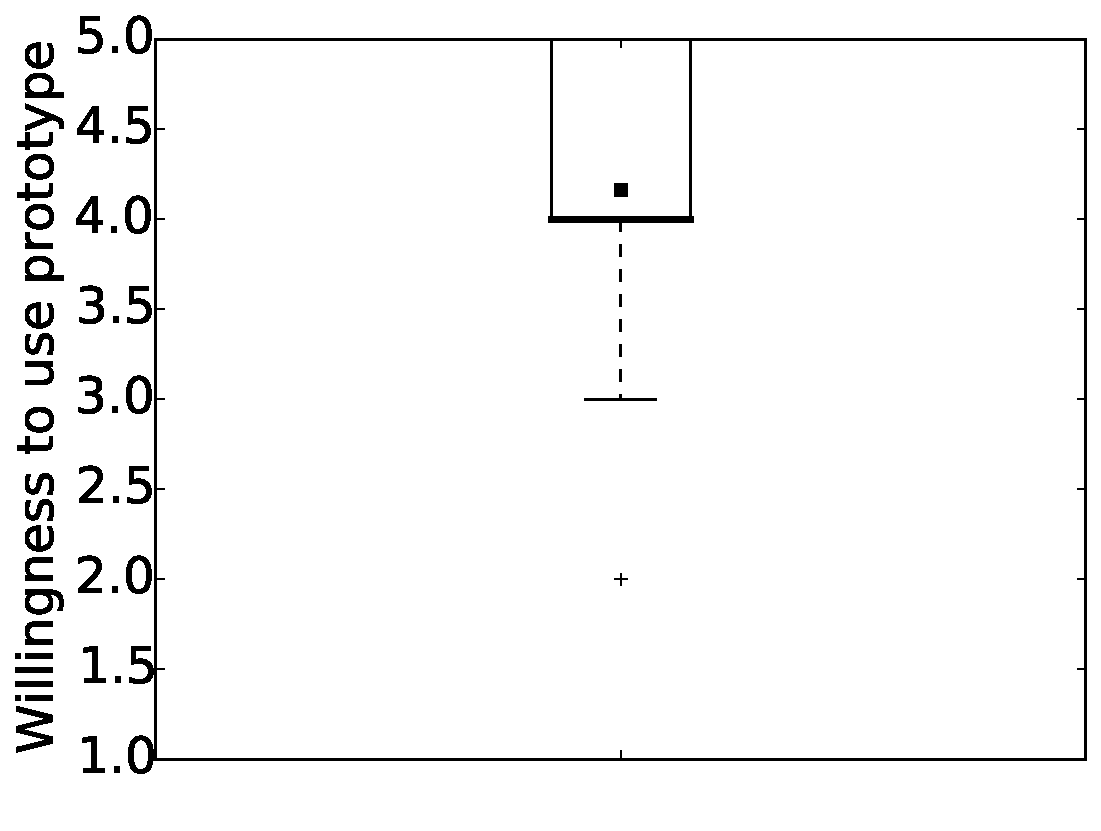
\includegraphics[width=\textwidth]{adinjection/figures/user_study/willingness.pdf}
        \caption{\scriptsize{Usability of content provenance.}}
        \label{adinjection:fig:eval:user_study:usability}
    \end{subfigure}
    \caption{User study results. For each boxplot, the box represents the
    boundaries of the first and third quartiles. The band within each box
    is the median, while the black square is the mean. The whiskers represent
    1.5 IQR boundaries, and outliers are represented as a \texttt{+} symbol.}
    \label{adinjection:fig:eval:user_study}
\end{figure}
